\documentclass[12pt]{article}

\usepackage{lipsum}
\usepackage{pgf-umlsd}
\usepackage[simplified]{pgf-umlcd}
\usepackage{float}
\usepackage{vhistory}
\usepackage{hyperref}
\usepackage{acro}
\usepackage{parskip}

\author{Tomislav Radanović, Rato Kuzmanić}
\title{Raccu Protocol Specification}
\date{\today}

\DeclareAcronym{sts}{
  short = STS,
  long  = secure token service,
  class = abbrev
}

\DeclareAcronym{ctap}{
  short = CTAP,
  long  = Client-to-Authenticator Protocol,
  class = abbrev
}

\begin{document}
    \begin{titlepage}
        \clearpage\maketitle
        \vfill
        \thispagestyle{empty}
    \end{titlepage}

    \clearpage\tableofcontents
    \thispagestyle{empty}
    \setcounter{page}{0}
    \newpage

    \section{Introduction}
This specification provides a formal, high-level overview of the Raccu protocol. 

    \subsection{Background}
    Raccu is a centralized \ac{sts} protocol for public-key cryptography authentication based on a 
    smartphone biometry. The protocol is architecturally inspired by the likes of OAuth 2.0, OpenID, 
    and W3C's WebAuthn while it conceptually resembles FIDO Alliance's \ac{ctap}, namely FIDO UAF standards. 

    \subsection{Goals}
    The core vision of Raccu is to provide a uniform method of authentication with the following properties: 
        \begin{enumerate}
            \item Smaller complexity and lesser cognitive load than in a traditional email and password 
                  authentication systems.
            \item Single registration process for authenticating to multiple web services and applications.
            \item Authentication process for issuing an attestation is independent of the type of registration 
                  used to create an account.
            \item Preserving data and origin integrity of the attestation through PKI based chain of trust.
            \item Requiring user's consent via independent biometric authorization process before granting an 
                  attestation.
        \end{enumerate}
    In the current version of the protocol, only an email-based registration is described in details, although 
    other types of registrations and verification claims can be easily added if needed.

    \subsection{Disclaimer}
    Implementation of certain elements of this specification may require licenses under third party intellectual 
    property rights, including without limitation, patent rights. The authors and any other contributors to this 
    specification are not, and shall not be held, responsible in any manner for identifying or failing to identify 
    any or all such third party intellectual property rights.    
    
    \medskip
    THIS SPECIFICATION IS PROVIDED “AS IS” AND WITHOUT ANY WARRANTY OF ANY KIND, INCLUDING, WITHOUT LIMITATION,
    ANY EXPRESS OR IMPLIED WARRANTY OF NON-INFRINGEMENT, MERCHANTABILITY OR FITNESS FOR A PARTICULAR PURPOSE.

    \subsection{Contributing}
    Anyone can contribute to the protocol or to its specification. To learn more about contributing, please visit our 
    official repository on GitHub located at \href{https://www.github.com/Raccu/Documentation}{https://www.github.com/Raccu/Documentation}.
    \newpage

    \section{Definitions}
Throughout the specification a following list of terms is widely used. In this section we define their meaning 
and what assumptions do we make on them.

\medskip
\textbf{Email}: Email client that allows the user to gain read access rights to the inbox associated
with the email address he/she provided. It is assumed that the user is the only person with the read access 
to this entity.

\medskip
\textbf{Auth}: Central authentication provider that serves as a secure token store (STS) and conforms to 
the Raccu Auth Provider API Specification. Valid and trusted certificate issued from the certificate authority (CA)
as a part of public key infrastructure (PKI) for this entity is implied.

\medskip
\textbf{Mobile}: A mobile application implementation conforming to the Raccu Mobile Application Specification 
that communicates with the corresponding Auth instance. Access to the fingerprint reader and an enabled biometric 
authentication on the host smartphone is implied.

\medskip
\textbf{Browser}: A client-side component in charge of rendering QR codes and dispatching appropriate messages 
as specified by this specification and a separate Raccu Client Component Specification. 

\medskip
\textbf{Attestation}: Digitally signed claim in a form of a token that confirms holder's identity. Issued by 
an Auth instance in a format defined in this specification and a separate Raccu Auth Provider API Specification. 
A secure storing of the attestation by its holder is implied.

\medskip
\textbf{Server}: An end web service or application that consumes an attestation issued by an Auth instance. 
Authorization service within the Server is assumed. Valid and trusted certificate issued as a part of PKI 
for this entity is implied.

\medskip
The key words "MUST", "MUST NOT", "REQUIRED", "SHALL", "SHALL NOT", "SHOULD", "SHOULD NOT", "RECOMMENDED", 
"MAY", and "OPTIONAL" in this specification are to be interpreted as described in 
\href{https://tools.ietf.org/html/rfc2119}{RFC 2119} and \href{https://tools.ietf.org/html/rfc8174}{RFC 8174}.
    \newpage

    \section{Register}
Registration is an act of sharing the proof of identity between the user and Auth. The proof of identity
can be in a specter of forms, including high confidence government issued documents and low confidence emails and 
phone numbers. Even though current version of Raccu protocol defines only email-based authentication, the protocol
has been designed with extensibility in mind, meaning that other types of verification claims can be added, if
needed.

      \subsection{Register via email}
      The flow of registering an account via email is shown in Figure~\ref{fig:registerViaEmail} on 
      page~\pageref{fig:registerViaEmail} and successful registration flow is defined as follows:
      \begin{enumerate}
            \item A user MUST provide a valid email.
            \item When Auth receives a valid registration request, email containing the verification code MUST 
                  be dispatched to the provided email address and a token returned to the Mobile.
            \item Upon receiving the verification code and entering it into the Mobile, the Mobile MUST provide 
                  a method to generate, store, and retrieve public key and an interface for signing an arbitrary 
                  message with the matching private key.
            \item Mobile MUST authenticate the user locally using a built-in biometry. Upon authenticating, 
                  the Mobile MUST finish an account creation by submitting a token, email, generated public key, 
                  and a digital signature of all of the previous parameters, with a REQUIRED addition of the 
                  verification code, to the Auth.
      \end{enumerate}
      \begin{figure}[H]
    \centering
    \begin{sequencediagram}

        \newinst{A}{Email}{}
        \newinst[3]{B}{Mobile}{}
        \newinst[3]{C}{Auth}{}
        
        \tiny
        \begin{call}{B}{POST /verify/email {(email)}}{C}{200 OK {(token)}}\end{call}{B}
        \mess{C}{Send an email {(verification code)}}{A}
        \mess{A}{verification code}{B}
        \begin{call}{B}{POST /register/email {(token, email, PU\textsubscript{k}, Sign{(token\textbar\textbar email\textbar\textbar PU\textsubscript{k}\textbar\textbar verification code)})}}{C}{200 OK}\end{call}{B}

    \end{sequencediagram}
    \caption{Register via email protocol flow.}
    \label{fig:registerViaEmail}
\end{figure}       
      If the registration via email fails for any reason related to the semantics of the protocol, an attempt to
      register MUST be discarded and all of the related data should be deleted. All of the following reasons are 
      considered to be a semantic of the protocol:
      \begin{itemize}
            \item Email is already associated with another account.
            \item Token does not exist.
            \item Token is not associated with a given email.
            \item Verification code entered into Mobile does not match the expected verification code.
            \item The signature cannot be verified by a given public key.
            \item The signature is invalid.
      \end{itemize}

    \newpage

    \section{Login}
    \lipsum[1]
    \subsection{Sequenced diagram}
    \begin{figure}[H]
        \centering
        \begin{sequencediagram}
            
            \newinst{A}{Mobile}{}
            \newinst[2]{B}{Web}{}
            \newinst[2]{C}{Auth}{}
            \newinst[2]{D}{Server}{}

            \tiny
            \begin{call}{B}{GET /resource/limited/1}{D}{401 Unauthorized}\end{call}{C}
            \begin{call}{B}{GET /auth}{C}{200 OK {(challenge)}}\end{call}{B}
            \mess{B}{QR{(challenge, domain)}}{A}
            \begin{call}{A}{POST /token {(challenge, email, domain, Sign{(...)})}}{C}{200 OK}\end{call}{A}
            \mess{C}{Confirmation successful}{B}
            \begin{call}{B}{GET /token/\{challenge\}}{C}{200 OK {(token)}}\end{call}{B}
            \begin{call}{B}{POST /login {(token)}}{D}{200 OK {(JWT, session cookie, ...)}}\end{call}{B}

        \end{sequencediagram}
        \caption{Login protocol flow}
    \end{figure}
    \subsection{Token}
    \lipsum[1]

    \begin{figure}[H]
        \centering
        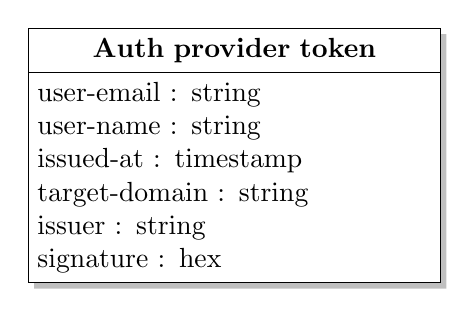
\begin{tikzpicture}
            \begin{class}[fill=white, drop shadow, draw=black]{Auth provider token}{0 ,0}
                \attribute{user-email : string}
                \attribute{user-name : string}
                \attribute{issued-at : timestamp}
                \attribute{target-domain : string}
                \attribute{issuer : string}
                \attribute{signature : hex}
            \end{class}
        \end{tikzpicture}
        \caption{Fields included into authentication token}
    \end{figure}

    \newpage

    \section{Reset creditentials}
    \lipsum[1]
    \subsection{Sequenced diagram}
    \begin{figure}[H]
        \centering
        \begin{sequencediagram}

            \newinst{A}{Email}{}
            \newinst[3]{B}{Mobile}{}
            \newinst[3]{C}{Auth}{}

            \tiny
            \begin{call}{B}{POST /reset {(email)}}{C}{200 OK}\end{call}{B}
            \mess{C}{Email{(code)}}{A}
            \mess{A}{code}{B}
            \begin{call}{B}{POST /reset/verify {(email, code)}}{C}{200 OK {(reset token)}}\end{call}{B}
            \begin{call}{B}{POST /reset/\{reset token\} {(reset token, PUk, Sign(...))}}{C}{200 OK}\end{call}{B}

        \end{sequencediagram}
        \caption{Reset creditentials protocol flow}
    \end{figure}
    \newpage

    \section{Delete account}
    \lipsum[1]
    \subsection{Sequenced diagram}
    \begin{figure}[H]
        \centering
        \begin{sequencediagram}

            \newinst{A}{Mobile}{}
            \newinst[5]{C}{Auth}{}

            \tiny
            \begin{call}{A}{DELETE / {(email, Sign{(...)})}}{C}{200 OK}\end{call}{A}
            
        \end{sequencediagram}
        \caption{Delete account protocol flow}
    \end{figure}
    \newpage

    \listoffigures\bigskip
    \printacronyms[include-classes=abbrev,name=Abbreviations]
    \begin{versionhistory}
        \vhEntry{0.0.0}{13.10.2018.}{Radanović}{Created document structure}
        \vhEntry{0.1.0}{18.10.2018.}{Radanović}{Added sequenced diagrams}
        \vhEntry{0.1.1}{23.10.2018.}{Radanović}{Updated sequenced diagrams}
        \vhEntry{0.2.0}{24.10.2018.}{Kuzmanić}{Added about project}
        \vhEntry{0.3.0}{25.10.2018.}{Kuzmanić}{Added introduction and definitions}
        \vhEntry{0.4.0}{25.10.2018.}{Kuzmanić}{Added registration via email}
    \end{versionhistory}
    
\end{document}
